% SIAM Article Template

\documentclass[review,hidelinks,onefignum,onetabnum]{siamart220329}
\newcommand{\bs}{\boldsymbol}
\newcommand{\eps}{\varepsilon}
\newcommand{\s}{\;}
\newcommand{\sif}{\text{ if }}
\newcommand{\pfrac}{\displaystyle \frac}
\newcommand{\Tau}{\mathcal{T}}
\newcommand{\Tref}{\mathcal{T}_{\text{ref}}}
\newcommand{\Qref}{\mathcal{Q}_{\text{ref}}}
\newcommand{\bb}[1]{\mathbb{#1}}

% Information that is shared between the article and the supplement
% (title and author information, macros, packages, etc.) goes into
% ex_shared.tex. If there is no supplement, this file can be included
% directly.

\input{ex_shared}

% Optional PDF information
\ifpdf
\hypersetup{
  pdftitle={A Numerical Method for Solving the Eikonal Eqauation on Simplicial Tesselations},
  pdfauthor={S. Natesh}
}
\fi

% The next statement enables references to information in the
% supplement. See the xr-hyperref package for details.

\externaldocument[][nocite]{ex_supplement}

% FundRef data to be entered by SIAM
%<funding-group specific-use="FundRef">
%<award-group>
%<funding-source>
%<named-content content-type="funder-name"> 
%</named-content> 
%<named-content content-type="funder-identifier"> 
%</named-content>
%</funding-source>
%<award-id> </award-id>
%</award-group>
%</funding-group>

\begin{document}

\maketitle

% REQUIRED
\begin{abstract}
In this paper, we describe a method for solving the Eikonal equation on domains in $\mathbb{R}^2$ or $\mathbb{R}^3$ tesselated by triangles or tetrahedra. Our method generalizes to simplices in higher dimensions, owing to our choice of solution representation under the Jacobi family of orthogonal polynomials on the simplex. First, we describe a spectral decomposition for functions supported on the simplex in terms of their weighted $L_2$ expansion coefficients under the Jacobi basis. Computing this expansion requires an accurate and efficient quadrature, and we provide a novel optimization routine based on approximate joint-diagonalization of Jacobi matrices for generating such quadratures. Then, we consider differential operators acting on coefficients of a Jacobi expansion. Recent results due to Townsend, Oliver and Vasil enable the construction of sparse differential operators on the standard triangle, interoperating within the Jacobi polynomial family parameter space, and leading to low-storage, banded discrete differential operators. We generalize these results to the tetrahedra (laying the path for generalizing to $d>3$), and use the resulting differential operators to construct the Eikonal operator on the simplex. Ultimately, we must solve a non-linear PDE, and working in coefficient space implies that our solution variables must be thought of as functions. Hence, we reformulate the Eikonal problem in terms of an infinite-dimensional $L_2$ mininization problem, which can be discretized with the aforementioned  numerical quadrature.
\end{abstract}

% REQUIRED
\begin{keywords}
multivariate orthogonal polynomials, spectral methods, partial differential equations, Eikonal equations, simplex
\end{keywords}

% REQUIRED
\begin{MSCcodes}
68Q25, 68R10, 68U05
\end{MSCcodes}

\section{Solutions to the Eikonal Equation}{}




\noindent Haven't really looked into the viscosity perspective, but..I think I converged on the same idea for solving the PDE. Consider the standard simplex $$\Tau^d = \{\bs{x}=(x_1,\cdots x_d)\in \bb{R}^d \s | \s x_i\geq 0,\s  1-|\bs{x}|_1 \geq 0\}$$

The \emph{minimal} time $u(x)$ to reach the boundary $\partial \Tau^d$ from a point $x\in \Tau^d$ is computable through solving the Eikonal equation on $\Tau^d$:
\begin{equation}\label{eq:eikonal}
	\begin{cases}
&\sum_{i = 1}^d (\partial_{x_i} u)^2 = \big(\frac{1}{f}^2\big),\quad x \in \Tau^d,\\
&u = q,\quad x \in \partial \Tau^d,
	\end{cases}
\end{equation}
where $f : \overline{\Tau^d} \to \bb{R}_\star^+$ is the speed in the medium, $q : \partial\Tau^d \to \bb{R}^+$ is the time to leave $\Tau^d$ from a point on $\partial\Tau^d$. Splitting \eqref{eq:eikonal} into homogeneous and particular problems lends itself well to numerical approximation with optimization libraries. As such, we can solve the problem in two steps. First, solve for $u_1$ in
\begin{equation}
	\begin{cases}
	&\sum_{i = 1}^d (\partial_{x_i} u_1)^2 = \big(\frac{1}{f}^2\big),\quad x \in \Tau^d
\end{cases}
\end{equation}
with no boundary constraints. Then, solve for $u_2$ in
\begin{equation}
	\begin{cases}
	&\sum_{i = 1}^d (\partial_{x_i} u_2)^2 = 0,\quad x \in \Tau^d\\
	&u_2 = q - u_1,\quad x \in \partial \Tau^d,
	\end{cases}
\end{equation}
with trivial RHS, and non-trivial boundary constraints.
Noting that the value of $u_1$ on the boundary is annihilated in the combined solution $$u=u_1+u_2,$$ we conclude that $u$  solves \eqref{eq:eikonal} 

We seek to represent $u$ under an optimal, finite, weighted $L_2$ expansion, wherein $$u(\bs{x}) \approx \sum_{j = 1}^n u_jP_j(\bs{x}) = \bs{u}\cdot \bs{P}(\bs{x}),$$
and $\bs{u}$ is the vector in $\bb{R}^n$ of coefficients of $u$ under the elements of the basis $\bs{P}(\bs{x}) : \bb{R}^d \to \bb{R}^n$. Here $\approx$ must be taken in the sense of weighted $L_2$ convergence of the series to $u$ as $n\to \infty$.

Let us specialize for $d=2$. By $P_k^n$, we denote the $k^{\text{th}}$ Jacobi polynomial on the triangle of degree $n$ with parameters $(a,b,c)$. When the parameters must be specified, we will refer to the same polynomial by $P_{k,n}^{(a,b,c)}$. The weight function is
\begin{equation}\label{eq:koornweight}
	\begin{split}
		W^{(a,b,c)}(x,y) &= x^{a-\frac{1}{2}}y^{b-\frac{1}{2}}(1-x-y)^{c-\frac{1}{2}},\\
		w_{(a,b,c)} &= \Big(\int_{\Tref^2}W(x,y)dxdy\Big)^{-1}=\frac{\Gamma(|\kappa| + \frac{3}{2})}{\Gamma(a+\frac{1}{2})\Gamma(b+\frac{1}{2})\Gamma(c+\frac{1}{2})} \\
		w^{(a,b,c)}(\bs{x}) &= w_{(a,b,c)}W^{(a,b,c)}(\bs{x})
	\end{split}
\end{equation}
with $a,b,c > -1/2$ the Jacobi parameters, and $|\kappa| = a+b+c$. The orthonormal polynomials are given in terms of the 1D Jacobi polynomials by
\begin{equation}\label{eq:koornwinder}
	\begin{split}
		P_k^n(x,y) &= (h_{k,n})^{-1}P_{n-k}^{2k+b+c,a-1/2}(2x-1)(1-x)^kP_k^{c-1/2,b-1/2}\Big(\frac{2y}{1-x}-1\Big),\\
		(h_{k,n})^2 &= \frac{w_{a,b,c}}{(2n+|\kappa|+\frac{1}{2})(2k+b+c)} \\
		&\times \frac{\Gamma(n+k+b+c+1)\Gamma(n-k+a+\frac{1}{2})\Gamma(k+b+\frac{1}{2})\Gamma(k+c+\frac{1}{2})}{(n-k)!k!\Gamma(n+k+|\kappa|+\frac{1}{2})\Gamma(k+b+c)},
	\end{split}
\end{equation}
and they satisfy a mutual orthonormality condition under the weighted inner product:
\begin{equation}\label{eq:koornorth}
	\langle P_j^m,P_k^n\rangle_W = \delta_{jk}\delta_{mn}. 
\end{equation}
That is to say, a given polynomial is not only orthonormal to those with different total degree, but also to those of the same degree. Notice, $P_k^n,\s0\leq k\leq n$ forms a basis for the space of homogeneous polynomials of degree $n$. By considering ordered collections of these subspaces, ordered by the degree $n$ of the space, instead of individual polynomials, we can more elegantly reformulate the Eikonal problem into a weak-type form. Let $$\bb{P}_n(x_1,x_2) = (P_0^n(x_1,x_2),\cdots P_n^n(x_1,x_2))^T,$$ and let $$\bs{P} = (\bb{P}_0^T,\bb{P}_1^T,\cdots,\bb{P}_{n-1}^T)^T.$$ The above notation amounts to a vectorization of the basis for the general space of polynomials in two variables $\Pi_{n-1}^2$ defined of $\Tau^2$.

Now, consider the $(n-1)$ order Jacobi polynomial expansion of the solution $u$ under the parameter family $(a,b,c)$. For $\bs{x} \in \Tau^d$, and $\text{dim}\Pi_{n-1}^2$ coefficients $\bs{u}$, we can write it as 
\begin{equation}
	u(\bs{x}) = \bs{P}^{a,b,c}(\bs{x})^T\bs{u}.
\end{equation}
There exists sparse discrete operators which map $\bs{u}$ to the coefficients of the derivative of $u$ under a modified basis, as well as those which promote the basis parameters without taking derivatives:
\begin{equation}
	\begin{split}
	\partial_{x_1} u(\bs{x}) &= \bs{P}^{(a+1,b+1,c+1)}(\bs{x})^T\mathcal{K}_{(a+1,b,c+1)}^{(a+1,b+1,c+1)}\mathcal{D}_{x_1}\bs{u}\\
	\partial_{x_2} u(\bs{y}) &= 
	\bs{P}^{(a+1, b+1,c+1)}(\bs{x})^T\mathcal{K}_{(a,b+1,c+1)}^{(a+1,b+1,c+1)}\mathcal{D}_{x_2}\bs{u}
	\end{split}
\end{equation}

Inserting this into the homogeneous constraint Eikonal equation gives
\begin{align}\label{eq:eikpdcoef}
	0 = &\big(\bs{P}^{(a+1,b+1,c+1)}(\bs{x})^T\mathcal{K}_{(a+1,b,c+1)}^{(a+1,b+1,c+1)}\mathcal{D}_{x_1}\bs{u}\big)^2 +\nonumber \\ &\big(\bs{P}^{(a+1, b+1,c+1)}(\bs{x})^T\mathcal{K}_{(a,b+1,c+1)}^{(a+1,b+1,c+1)}\mathcal{D}_{x_2}\bs{u}\big)^2 \nonumber \\
	=
	 &\bs{P}^{(a+1,b+1,c+1)}(\bs{x})^T\big(\mathcal{\tilde{D}}_{x_1}\bs{u}\bs{u}^T\mathcal{\tilde{D}}_{x_1}^T + \mathcal{\tilde{D}}_{x_2}\bs{u}\bs{u}^T\mathcal{\tilde{D}}_{x_2}^T \big)\bs{P}^{(a+1,b,c+1)}(\bs{x}),
\end{align}
where $$\mathcal{\tilde{D}}_{x_1} = \mathcal{K}_{(a+1,b,c+1)}^{(a+1,b+1,c+1)}\mathcal{D}_{x_1},$$ and $$\mathcal{\tilde{D}}_{x_2} = \mathcal{K}_{(a,b+1,c+1)}^{(a+1,b+1,c+1)}\mathcal{D}_{x_2}.$$ The above equality holds for any point $\bs{x}\in \Tau^2$. So, for a solution $\bs{u}$, the coefficient operation must be identically zero:
\begin{equation}\label{eq:eikdcoef}
	\big(\mathcal{\tilde{D}}_{x_1}\bs{u}\bs{u}^T\mathcal{\tilde{D}}_{x_1}^T + \mathcal{\tilde{D}}_{x_2}\bs{u}\bs{u}^T\mathcal{\tilde{D}}_{x_2}^T \big) \equiv 0.
\end{equation}
 Now, we seek a coefficient solution $\bs{u}$ which represents the solution \emph{globally} in $\Tau^2$. However, polynomials are differentiable, and some of the problems we are interested in yield non-differentiable solutions. This is true even in the most basic case of $f \equiv 1$, in which $u$ is the signed distance function from $\bs{x}$ to $\partial\Tau^2$, depicted below:

\begin{figure}[H]
	\centering
	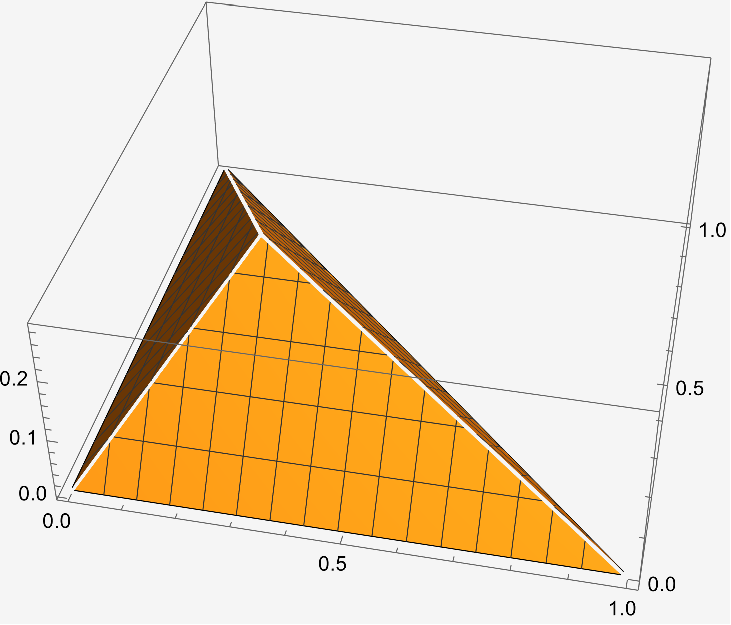
\includegraphics[width=0.75\linewidth]{./distT2}
	\caption{A simple calculation shows that the minimum distance from $\bs{x}\in\Tau^2$ to the boundary $\partial\Tau^2$ is given by the minimum of $\Big\{x_1,x_2,\Big|\Big|\bs{x}-\begin{bmatrix}
	(x_1-x_2 + 1)/2 \\ (x_2-x_1+1)/2
	\end{bmatrix}\Big|\Big|_2\Big\}$}\label{fig:distT2}
\end{figure}
We cannot hope to recover a solution $\bs{u}$ which  satisfies \eqref{eq:eikdcoef} to machine precision, as that would imply the global solution has zero residual \emph{pointwise} everywhere. Hence, we must return to \eqref{eq:eikpdcoef}, and consider solving it weakly, in the sense of:
\begin{equation}\label{eq:eikonalweak}
	\begin{split}
		0&\approx\\
\int_{\Tau^2}w^{(a+1,b+1,c+1)}&(\bs{x})\bs{P}^{(a+1,b+1,c+1)}(\bs{x})^T\big(\mathcal{\tilde{D}}_{x_1}\bs{u}\bs{u}^T\mathcal{\tilde{D}}_{x_1}^T + \mathcal{\tilde{D}}_{x_2}\bs{u}\bs{u}^T\mathcal{\tilde{D}}_{x_2}^T \big)\bs{P}^{(a+1,b+1,c+1)}(\bs{x})d\bs{x}\\
&\approx ||\partial_x u||_{w^{(a+1,b+1,c+1)}}^2 +  ||\partial_y u||_{w^{(a+1,b+1,c+1)}}^2.
	\end{split}
\end{equation}
That is, we seek to minimize the square of the gradient norm, where the squared norm is viewed as a function in $L^2(\Tau^2,w^{(a+1,b+1,c+1)})$. Incorporating non-zero RHS of the Eikonal problem amounts to subtracting the outer-product of coefficients (promoted to $(a+1,b+1,c+1)$ ) of $(1/f)$ from the constant vector parenthetical term in \eqref{eq:eikonalweak}.

Parsing this equation out a bit further (condensing sub/super scripts), we have
\begin{align*}
&=\int_{\Tau^2} \bs{P}(\bs{x})^T (\bs{u_x}\bs{u_x}^T + \bs{u_y}\bs{u_y}^T)w(\bs{x})\bs{P}(\bs{x})d\bs{x}\\
&=\int_{\Tau^2}\bs{P}(\bs{x})^T 
\begin{bmatrix}
	 u_{x,1}^2 & u_{x,1}u_{x,2} & \cdots & u_{x,1}u_{x,N}\\
	 u_{x,2}u_{x,1} & u_{x,2}^2 & \cdots & u_{x,2}u_{x,N}\\
	 \vdots & \ddots&\ddots \\
	 u_{x,N}u_{x,1} & u_{x,N}u_{x,2} & \cdots & u_{x,N}^2
\end{bmatrix}\bs{P}(\bs{x})w(\bs{x})d\bs{x} \\
&= \int_{\Tau^2}
 \begin{bmatrix}
	P_1(\bs{x}) & P_2(\bs{x}) & \cdots & P_N(\bs{x})
\end{bmatrix}
\begin{bmatrix}
u_{x,1}^2 & u_{x,1}u_{x,2} & \cdots & u_{x,1}u_{x,N}\\
u_{x,2}u_{x,1} & u_{x,2}^2 & \cdots & u_{x,2}u_{x,N}\\
\vdots & \ddots&\ddots \\
u_{x,N}u_{x,1} & u_{x,N}u_{x,2} & \cdots & u_{x,N}^2
\end{bmatrix}
\begin{bmatrix}
P_1(\bs{x}) \\ P_2(\bs{x}) \\ \vdots \\ P_N(\bs{x})
\end{bmatrix}w(\bs{x})d\bs{x}
\end{align*}

There are some errors above which I need to address.

%The remaining integral term should result in the identity matrix of size $\text{dim}\Pi_{n-1}^2$ by the orthonormality relations. If the promotion matrices for the derivatives weren't handled correctly, this might be the source of my problems..and I may need to multiply the constant outer product term by some weights. All of this is to say that when looking at errors for convergence analysis, I need to make sure to look at my own stated definition for $\approx$, i.e. in the weighted $L_2$ sense..

\section{A variational approach}
Let's try framing the problem from the perspective of infinite dimensional optimization. Thus far, my efforts have fallen under the discretize-then-optimize approach for solving non-linear PDEs. So, let's flip that and consider the optimize-then-discretize approach. 

We want to solve
\begin{equation}
	\begin{split}
	\min_{u\in L_2(\Tau^2,w^{(a,b,c)})}\mathcal{L}(u),\\
	\text{s.t. } u = q \text{ on } \partial\Tau^2
	\end{split},
\end{equation}
where $\mathcal{L}$ is defined by 
\begin{equation}
	\mathcal{L}(u) := \int_{\mathcal{T}^2}\big( |\nabla_{\bs{x}} u|^2 - 1 \big) d\bs{x}
\end{equation}

The steps here are to derive the first variation of $\mathcal{L}$ as $$\delta\mathcal{L}(u,\hat{u}) = \partial \varepsilon\mathcal{L}(u+\varepsilon \hat{u})|_{\varepsilon=0} = 0,$$ where $\hat{u} \in \mathcal{H}_0^1(\Tau^2)$. This gives the necessary condition a minimizer of $\mathcal{L}$ must satisfy. Then, compute the second variation by considering another $\tilde{u} \in \mathcal{H}_0^1$, and deriving the newton step through $$\delta^2 \mathcal{L}(u,\hat{u},\tilde{u}) = \partial_\varepsilon\delta \mathcal{L}(u+\varepsilon \tilde{u},\hat{u})$$ and find the step direction by solving 
$$\delta^2 \mathcal{L}(u^k)(\hat{u},\tilde{u}) = -\delta\mathcal{L}(u^k)(\hat{u}),\quad \forall \hat{u} \in \mathcal{H}_0^1$$
By choosing $u^0 = q$ on $\partial \Tau^2$, and setting $u^{k+1} = u^k + \tilde{u}$, we have an infinite-dimensional newton stepper for solving the Eikonal problem. I'm not sure I like where this goes in terms of complexity (mental and computational), so will stick to the DTO approach for now. There is also probably a correct energy functional which gives the Eikonal problem, which is likely not the one I started with.
%\bibliographystyle{siamplain}
%\bibliography{references}
\end{document}
